\chapter{Guide}
In this section I am going to discuss the various pages of the app, 
I am also going to give a brief description of the various components in each page,
and how the user can interact with them.
Note that some of the details (and images) in this section are subject to minor changes.
%%%%%%%%%%%%%%%%%%%%%%%%%%%%%%%%%%%%%%%%%%%%%%%%%%%%%%%%%%%%%%%%%%%%%%%%%%%%%%%%%%%
\section{Home Screen}
The home page of this app contains a list of topics in black, 
organized by type of algorithm. 
These topics are among those covered in an intermediate Algorithms class. 
The topics that have been covered are in blue instead of black,
and they are links that lead to their corresponding page. 
The purpose of this page is to show a list of potential future additions 
to this project. 
The navigation bar also has links to each problem that is covered by the project. 
	\begin{figure}[h]
		\caption{Home Page}
		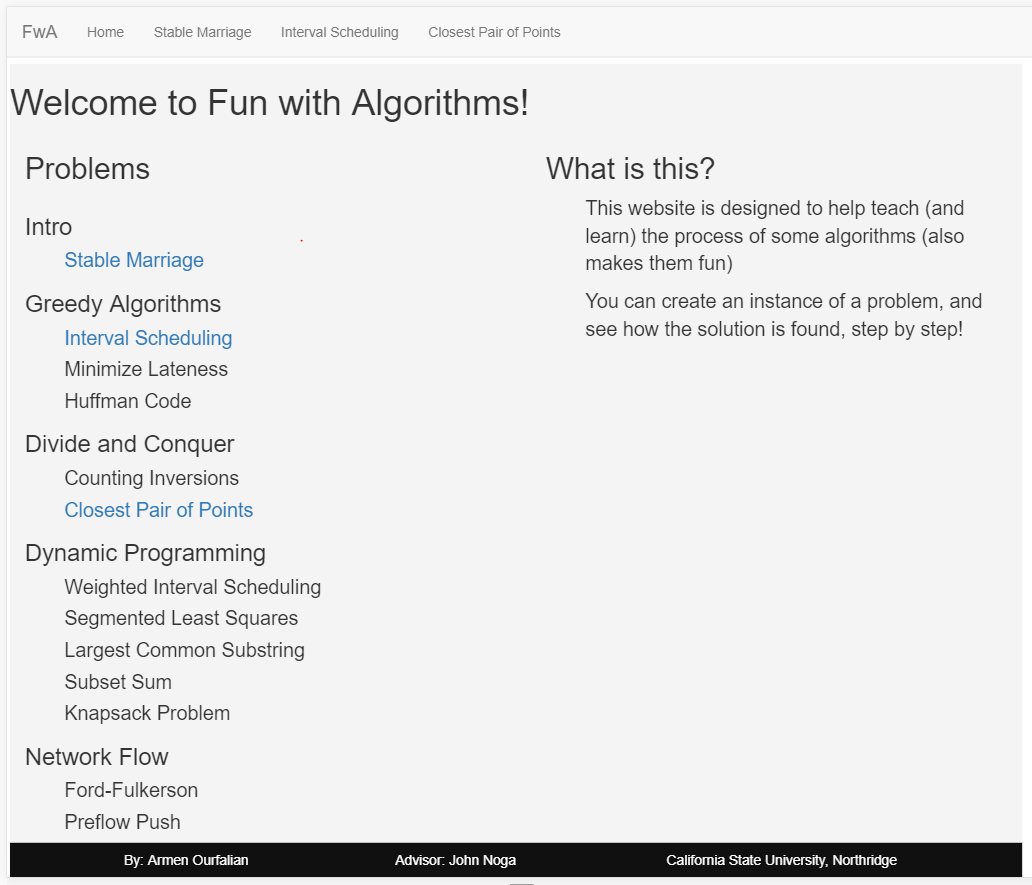
\includegraphics[
			height = 3in
		]{images/home-screen.png}
		\centering
	\end{figure}
%%%%%%%%%%%%%%%%%%%%%%%%%%%%%%%%%%%%%%%%%%%%%%%%%%%%%%%%%%%%%%%%%%%%%%%%%%%%%%%%%%%
\section{Reusable Components}
As mentioned in \textbf{Chapter \ref{tools-and-technologies} Tools and Technologies}, 
a key feature of Vue is reusable components. So a number of components in this app 
were created with reusability in mind. 
Reusing the same components across various pages gives the website 
a more consistent interface overall. 
This also lessens the learning curve required to use this app.
I packed the majority of the reausable functionalities into the secondary 
navigation bar to ensure they would be easy to find no matter what page the 
user found themselves on. 
The key features of the second navbar are the following: 
\begin{figure}[h]
	\caption{Second Navbar}
	
\includegraphics[
	width = \textwidth
	]{images/second-nav.png}
	\label{fig-second-nav}
	\centering
\end{figure}
\newline\newline
A \textbf{File Menu} with the options \textit{Save as Text} and \textit{Load as Text}. 
These features are familiar to the modern user. 
Although the interface to save or load an instance is exactly the same For each problem,
the save and load functionalities are customized for each problem. 
This is because each problem requires a different format for its input data.
\newline\newline
For example: \textsc{Stable Marriage} requires an input of exactly two $n\times n$
lists of numbers, where the numbers 
must be in the range $[0, n-1]$ or $[1, n]$, 
whereas the \textsc{Interval Scheduling} 
requires an input of any number of rows, each containing two numbers.
Despite these differences, the interface for saving or loading instances 
is exactly the same for all problems within the entire project. 
\begin{figure}[h]
	\caption{File Menu}
	
\includegraphics[
	]{images/file-menu.png}
	\label{fig-file-menu}
	\centering
\end{figure}
\newline\newline
An \textbf{Examples Menu} that contains a list of 
pre-made instances for each problem that are loaded from a database.
\begin{figure}[h]
	\caption{Examples Menu for Stable Marriage}
	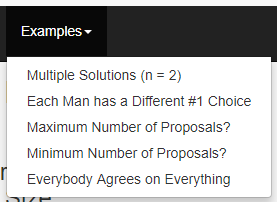
\includegraphics[
	]{images/example-menu.png}
	\label{fig-example-menu}
	\centering
\end{figure}
\newline\newline
A switch to go between \textbf{Edit Mode} and \textbf{Solve Mode}. 
Edit Mode will display the \textsc{Instance Maker},
whereas Solve Mode will display the \textsc{Solver}. 
In both modes, the \textsc{Display} will also be visible. 
\begin{figure}[h]
	\caption{Edit Mode}
	\label{fig-edit-mode}
	
\includegraphics[]{images/edit-mode.png}
	\centering
	\caption{Solve Mode}
	\label{fig-solve-mode}
	
\includegraphics[]{images/solve-mode.png}
	\centering
\end{figure}
\newline\newline
The functionality of this switch is the same across all problems within the app:
the problem instance can only be changed when the page is on Edit Mode, 
and algorithm can only be performed while in Solve Mode. 
The reason for this is because giving the user the ability to change the 
problem instance mid-way through the algorithm would cause unexpected problems
such as infinite loops or divide-by-zero errors. 
For this reason, whenever the user switches from Solve Mode into Edit Mode, 
the \textsc{Solver} is completely reset to its initial state, and any progress
made in the algorithm is lost.
%%%%%%%%%%%%%%%%%%%%%%%%%%%%%%%%%%%%%%%%%%%%%%%%%%%%%%%%%%%%%%%%%%%%%%%%%%%%%%%%%%%
\section{Stable Marriage}
%%%%%%%%%%%%%%%%%%%%%%%%%%%%%%%%%%%%%%%%%%%%%%%%%%%%%%%%%%%%%%%%%%%%%%%%%%%%%%%%%%%
\section{Interval Scheduling}
%%%%%%%%%%%%%%%%%%%%%%%%%%%%%%%%%%%%%%%%%%%%%%%%%%%%%%%%%%%%%%%%%%%%%%%%%%%%%%%%%%%
\section{Closest Pair of Points}